\section{Introduction}

\begin{frame}
\frametitle{Definitions}
\begin{itemize}
\item  Set of agents $N$ \\
\centering
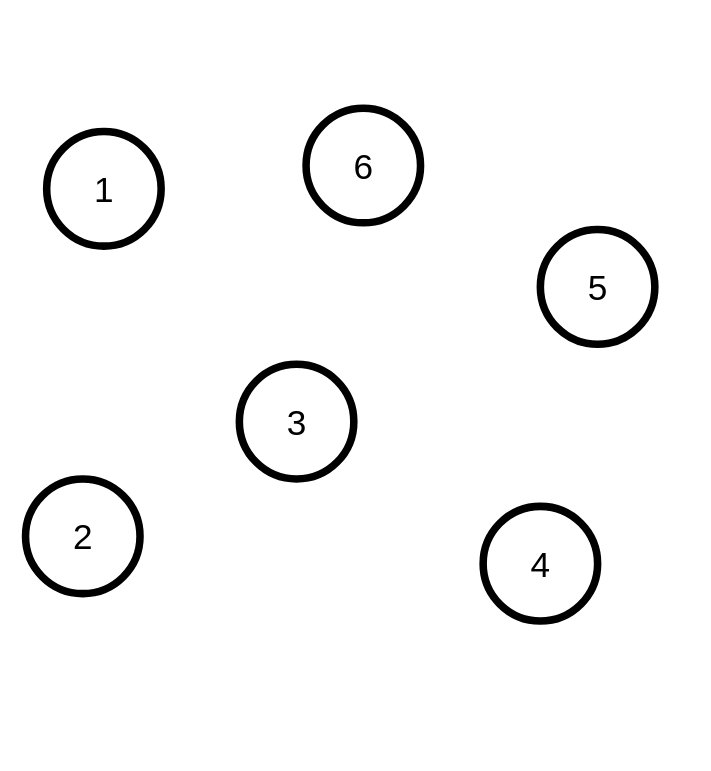
\includegraphics[width=5cm]{img/intro/agents.png}
\end{itemize}
\end{frame}



\begin{frame}
\frametitle{Definitions}
\begin{itemize}
\item Outcomes $O$ \\
\centering
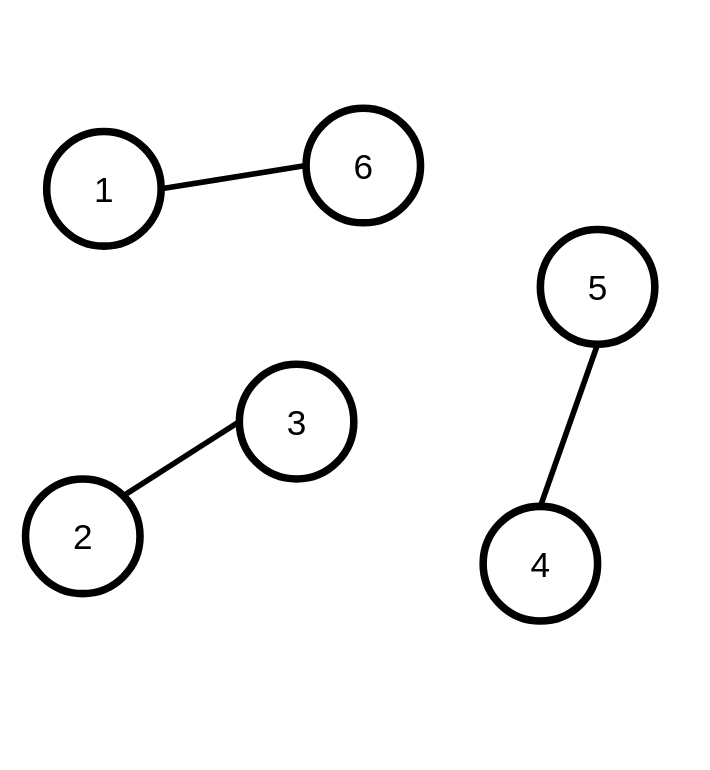
\includegraphics[width=5cm]{img/intro/agents_matched.png}
\end{itemize}
\end{frame}

\begin{frame}
\frametitle{Definitions}
\begin{itemize}
\item Outcomes $O$ \\
\centering
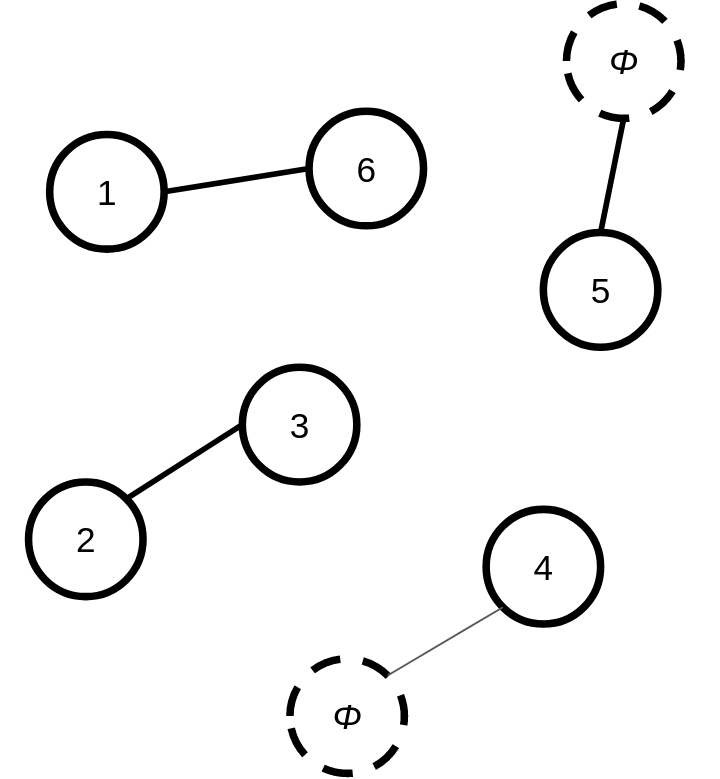
\includegraphics[width=5cm]{img/intro/agents_unmatched.png}
\end{itemize}
\end{frame}


\begin{frame}
\frametitle{Definitions}
\begin{itemize}[<+->]
\item Preference orders $\succeq_i \in R$
\item Preference profile $\succeq := (\succeq_1,\ldots, \succeq_n) \in R^n$
\item Reported preferences $\hat{\succeq}$
\item Mechanism with rules $g$, while $g(\hat{\succeq}) = o \in O$
\end{itemize}
\centering
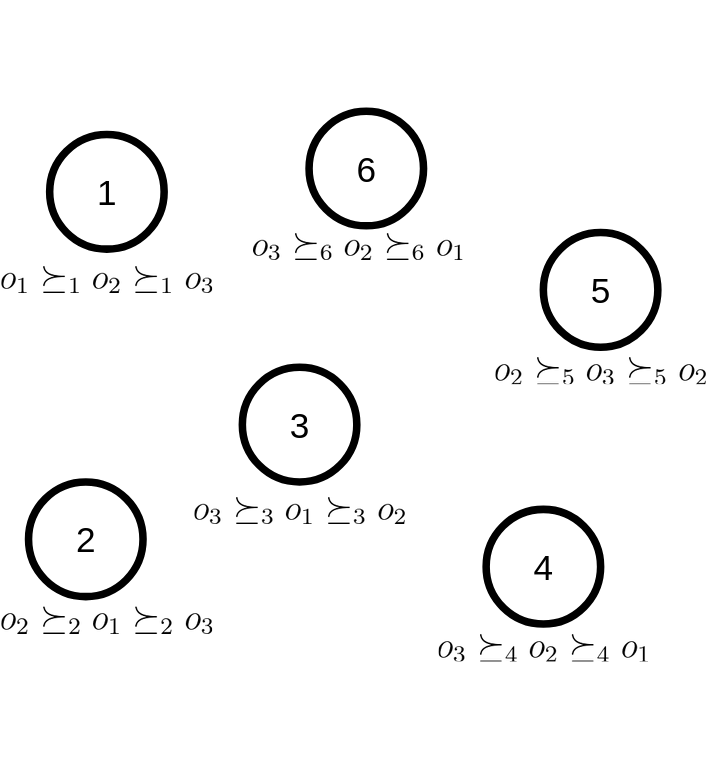
\includegraphics[width=7cm]{img/intro/agents_preferences.png}
\end{frame}


\begin{frame}
\frametitle{Mechanism properties}
\begin{itemize}[<+->]
\item onto
\item dictatorial
\item dominant strategy
\item strategy-proof
\end{itemize}
\end{frame}

\begin{frame}
\frametitle{Gibbard-Satterthwaite impossibility}
In a domain with three or more outcomes and where all strict preference orders on outcomes are possible, an \textbf{onto} and \textbf{strategy-proof} mechanism is \textbf{dictatorial}. \\
(Parkes and Seuken)

\end{frame}

\begin{frame}
\frametitle{Assumptions}
\begin{itemize}[<+->]
\item Agents are indifferent about parts of the matching, in which they are not directly involved
\item Payments are not available 
\item Simultaneous move game, agents report preferences simultaneously

\end{itemize}
\end{frame}